%
% clip.tex
%
% (c) 2024 Lukas Schöpf, OST Ostschweizer Fachhochschule
%

% DeepL corrected
% explain Resnet and transformer

\chapter{Cross-modal networks
    \label{chapter:crossmodalnetworks}}
    Multimodal deep learning is the study of models that learn from multiple modalities.
    For example, a human can use both vision and hearing to identify an object or a person.
    Cross-modal deep learning uses data from one modality to improve performance in another.
    For example, if a person looks at a picture of a bird and listens to the bird's song, they might be able to identify the bird.
    
    Its most impressive feature is the ability to perform well on data on which the model has not been trained.
    This ability is called zero-shot capability, which is derived from N-shot capability.
    N-shot capability describes how many training samples of a particular class a model needs to classify it correctly.

    In this work, cross-modal networks are used to find relationships between images and text.
    Networks trained for this task are called contrastive language-image pre-training models.
    Most cross-modal networks built for this task consist of a text encoder and an image encoder.

    \section{Base networks}
    To understand corss-modal netwroks we first have to understand thier components.
    Most of them use a transformers as encoders but some can use ResNets.
    
    \subsection{ResNet}
    ResNet's were introduced in \cite{resnetpaper}.
    A ResNet uses residual blocks (\cref{fig:crossmodalnetworks:resblock}).
    These blocks have residual conections between some layers.
    This allows information to bypass whole layers if the layers are not needed.
    These conections stabilizes training and convergence of deep neural networks.
    Big and deep transformer models like GPT models from Open AI use these conections.

    \begin{figure}[h]
        \centering
        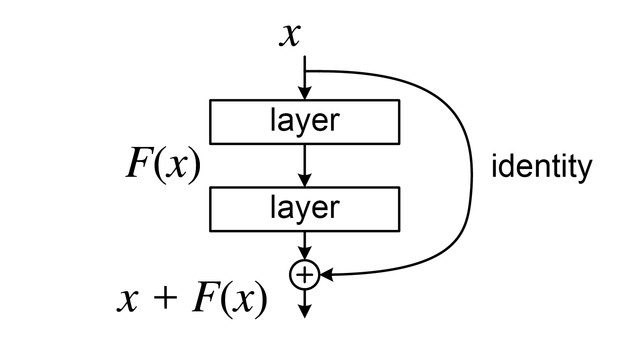
\includegraphics[width=0.55\textwidth]{Images/crossmodalnetworks/ResBlock.png}
        \caption{Image of a ResNet block.\cite{resnetpaper}}
        \label{fig:crossmodalnetworks:resblock}
    \end{figure}

    \subsection{Transformer}

    The transformer is first meantioned in \cite{attentionisallyouneed}.
    Before transformers \acrfull{rnn} were used to process sequential data.
    A mechanism called attention was used to get information about the context of a sequenz.
    The transformer was a revolution because it uses a  block called self attention.
    With this block the need for a \acrshort{rnn} is obsolet.
    \acrshort{rnn} are hard to train because of a effect called vanishing or exploding gradient.
    They are also hard to parallelize.
    These effect's no longer occure when using a transformer.

    \begin{figure}[h]
        \centering
        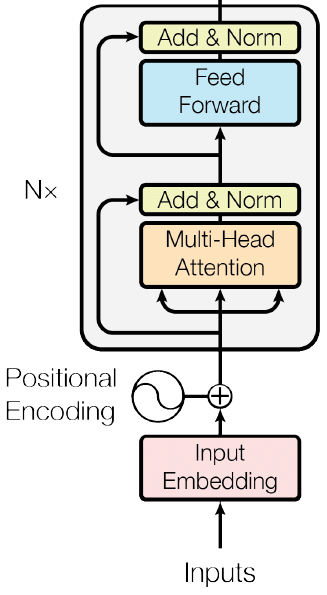
\includegraphics[width=0.25\textwidth]{Images/crossmodalnetworks/The-Transformer-encoder-structure.png}
        \caption{Image of a transformer which in the case of CLIP is used as a text encoder\cite{fig:encoder}}
        \label{fig:crossmodalnetworks:transformer}
    \end{figure}

    



    \section{Text encoder}
    The text encoder is in most cases a transformer.
    It encodes a given text into a high-dimensional vector space.
    This high dimensional vector space allows the encoder to correctly classify unseen classes because their vector is close to related classes.
    In theory, the closer two words are related, the closer their embedding vectors are to each other.
    An example of this can be seen in \cref{fig:crossmodalnetworks:3demb}, where \Acrfull{pca} is used to reduce the dimensions of the embedding vectors.
    Cat and dog are close together.

    \begin{figure}
        \centering
        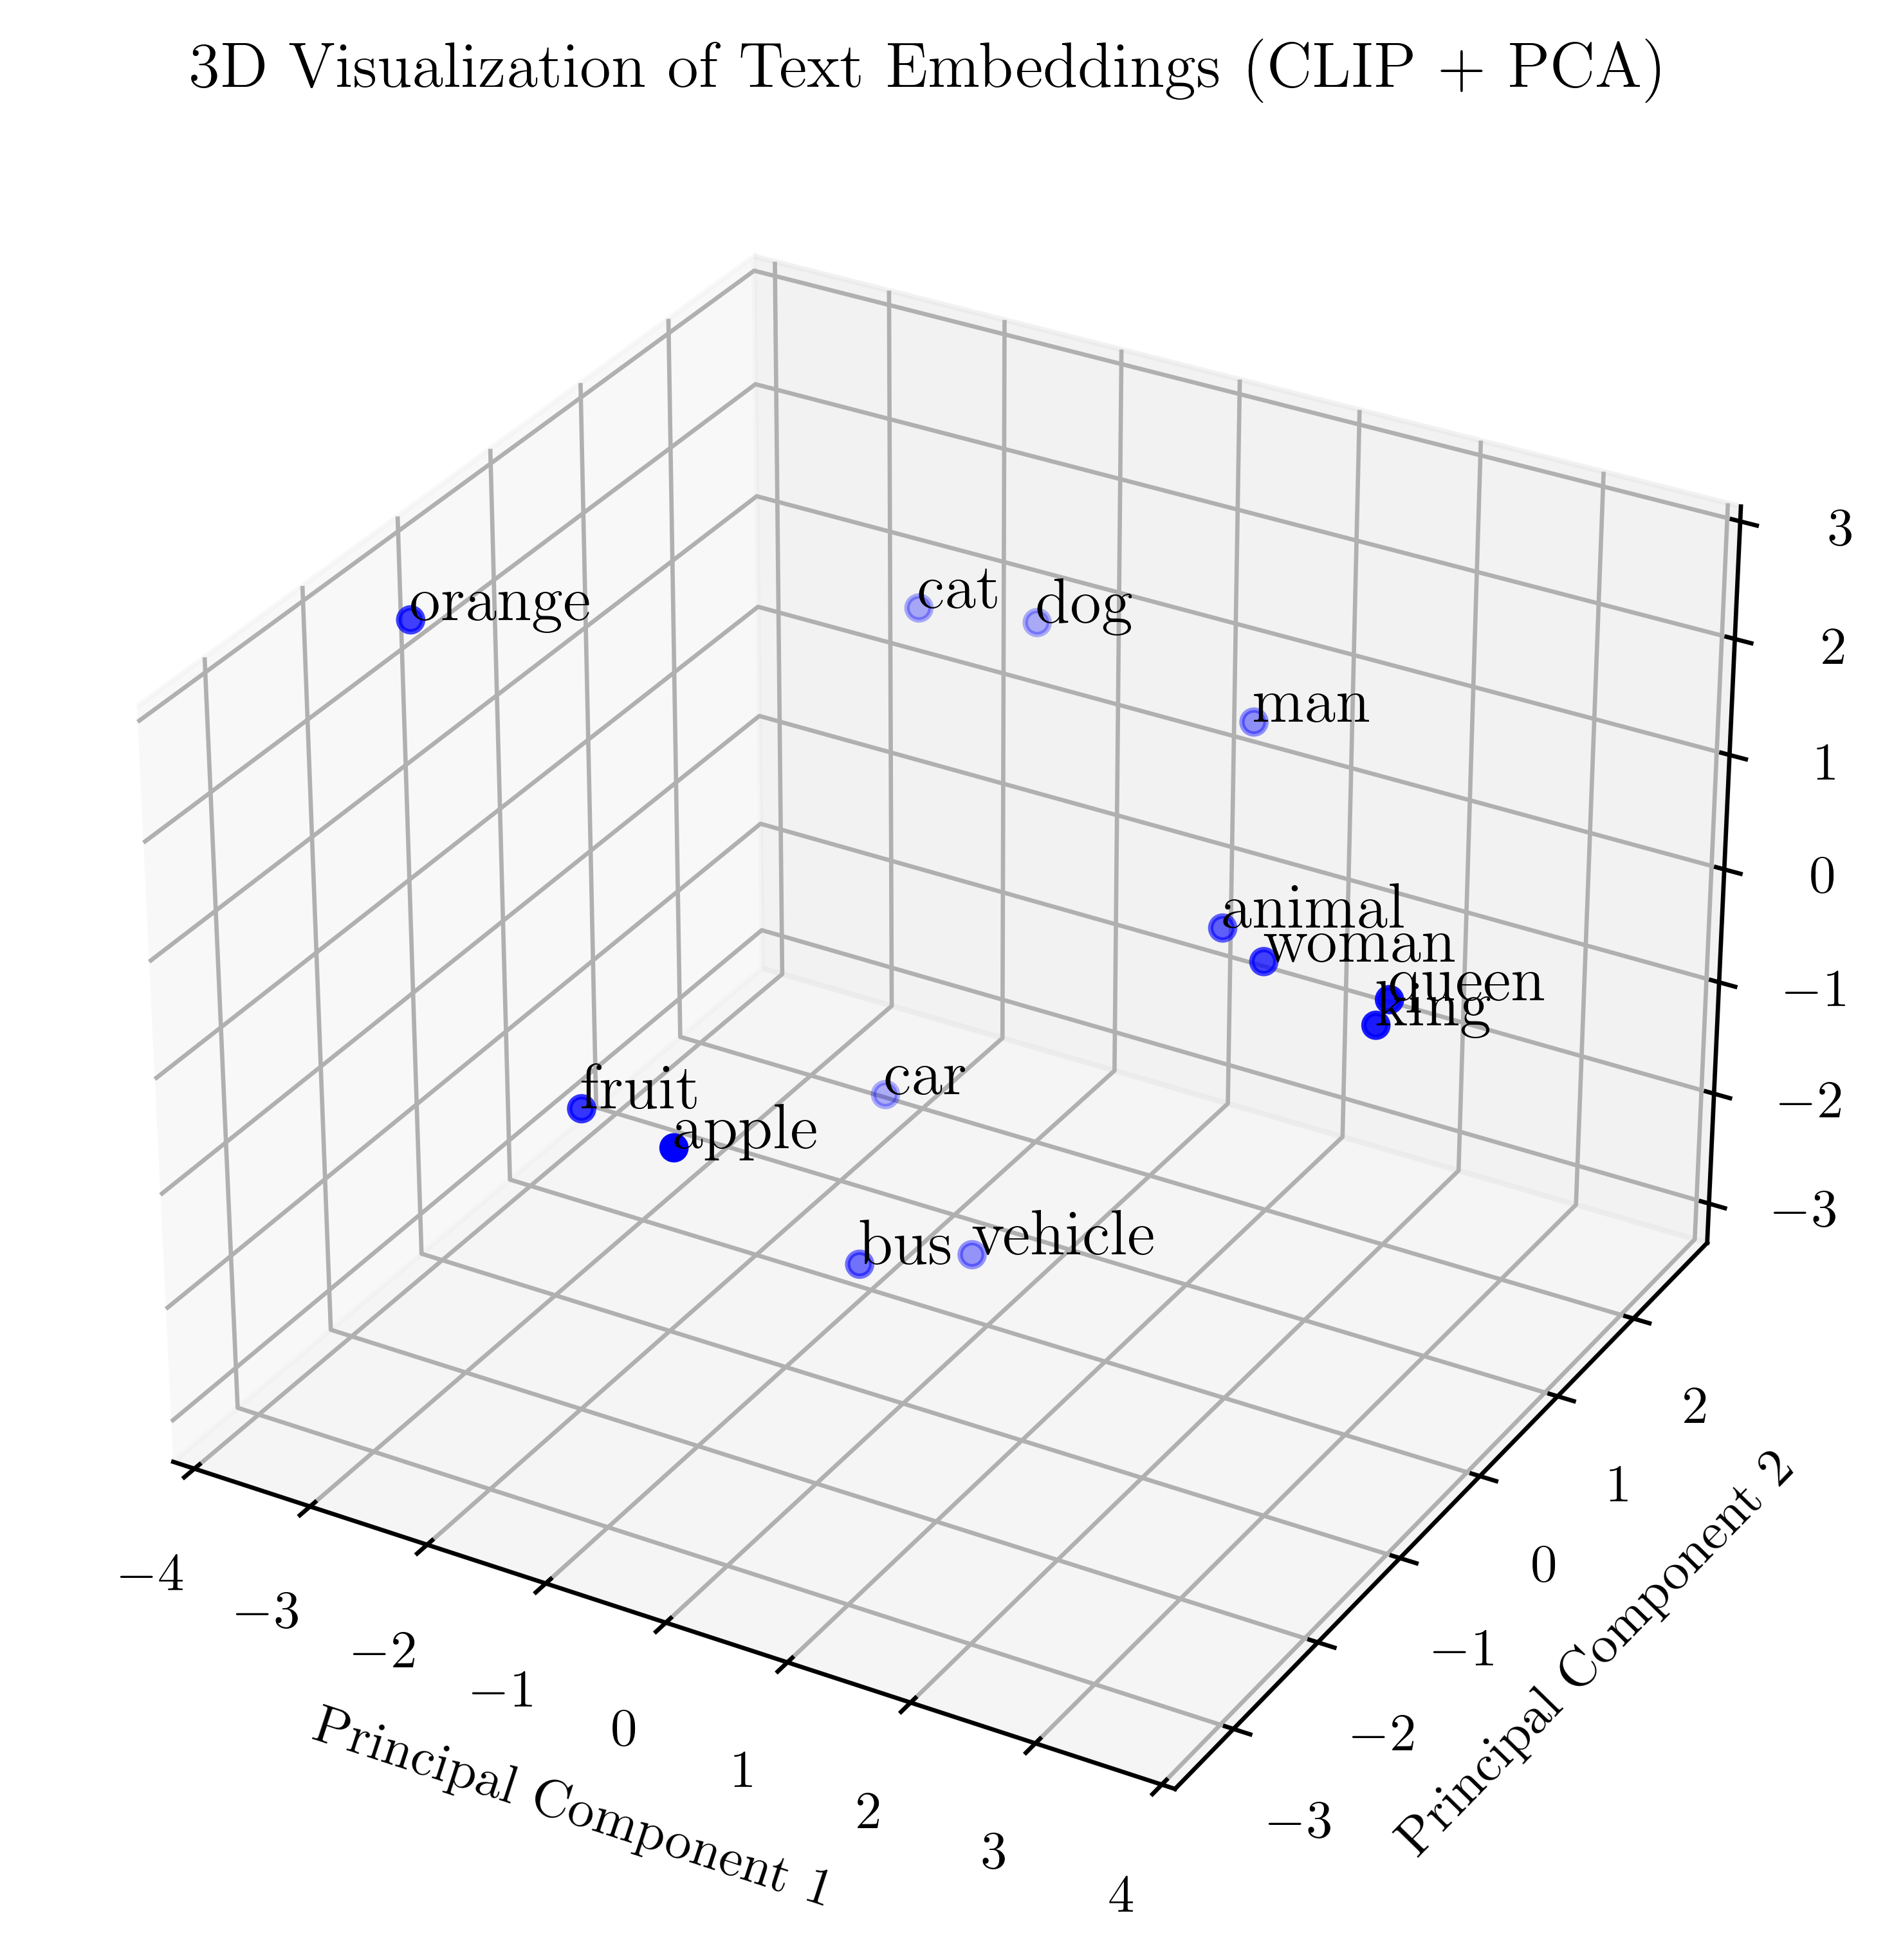
\includegraphics[width=\textwidth]{Images/crossmodalnetworks/3DEmbedding.png}
        \caption{Example of text embedding using CLIP and \Acrshort{pca}}
        \label{fig:crossmodalnetworks:3demb}
    \end{figure}
    
    \section{Image encoder}
    In most cases, the image encoder consists of a vision transformer\cite{Vis_N_Grams}.
    Like a text encoder, the vision encoder encodes an image in a high-dimensional vector space.
    A vision transformer needs an image in a specific dimension.
    For this reason, an image encoder is a pair of vision transformer and preprocessor that transforms an image into the right dimensions for the vision transformer.

    
    \section{Contrastive Language-Image models
        \label{section:languageimagemodels}}
        This section examines some models that use contrastive language-image pretraining.
        Most of the information in this section is taken from \cite{cliplikeweb} and the related papers.

        Contrastive techniques take paired inputs from two modalities (e.g. an image and its caption).
        Both inputs are embedded in their own embedding space.
        The aim is for such a pair to be represented by its corresponding encoder in a similar embedding.
        Speech-image describes the two modalities used by a model.
        Pre-training means that the model has been trained on a large and universal dataset.
        These models are often called basic models.
        For a specific application, a pre-trained model can be fine-tuned to better perform its specific task.

        \subsection{CLIP
            \label{section:clip}}
        \acrfull{clip} \cite{clip} is a cross-modal model from openAI\cite{openai} that can tell how well a given image and text match.
        It can be used with a variety of image and text encoders.
        It is trained on a large dataset consisting of 400 million image-text pairs.
        It has been shown to outperform some of the best known models in classifing images.
        Many other models use CLIP as a base and build better models from it.

        \begin{figure}[!h]
            \centering
            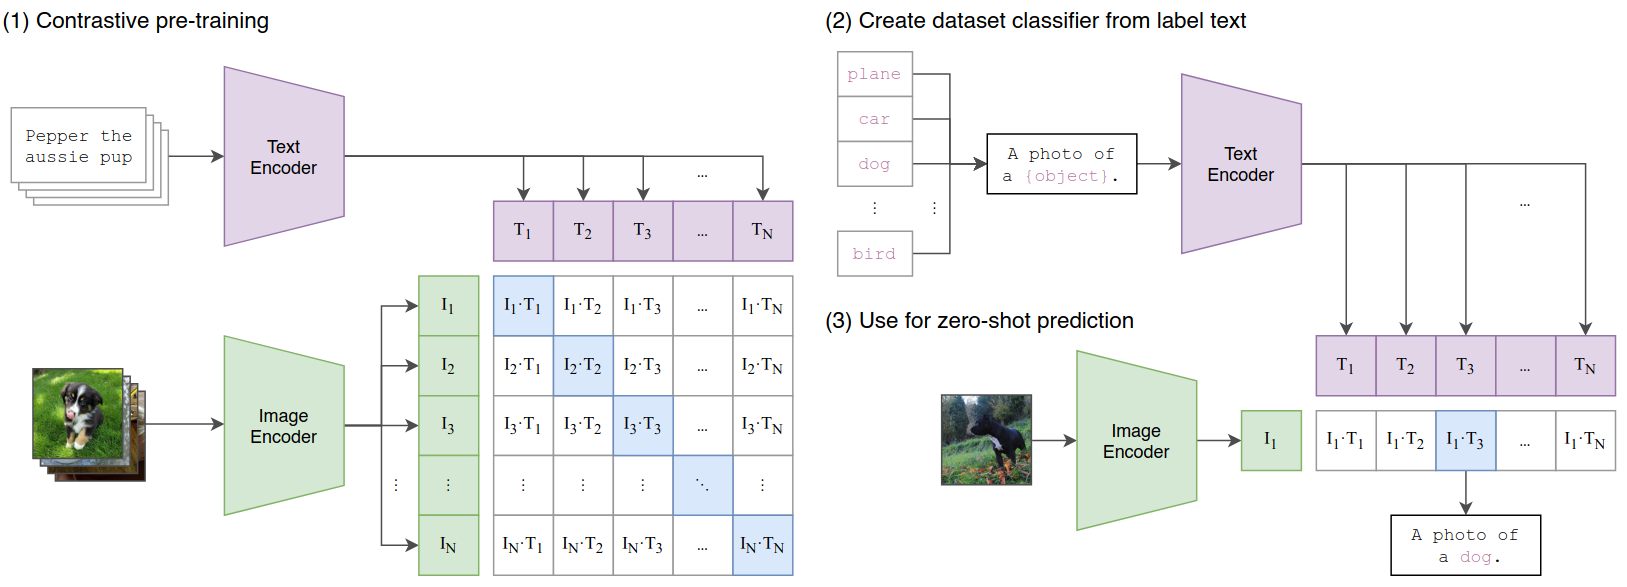
\includegraphics[width=\textwidth]{Images/crossmodalnetworks/OpenAICLIP.png}
            \caption{A picture from the \acrshort{clip} paper by OpenAI \cite{clip}.}
            \label{fig:crossmodalnetworks:openaiclip}
        \end{figure}

        \subsection{ALIGN
            \label{section:align}}
        \acrfull{align}\cite{ALIGN} was released shortly after \acrshort{clip}.
        Rather than relying on small and image caption datasets, \acrshort{align} uses a dataset of \(1.8\) billion pairs of image and alt-text pairs (e.g. in \cref{fig:crossmodalnetworks:alignepairs}).
        These alt-text descriptions are much noisier than captions.
        The authors apply basic filtering to remove duplicates, images with more than 1000 associated alt-texts, and uninformative alt-texts (either too frequent or containing rare tokens), but avoid expensive filtering operations.
        With just these simple steps, ALIGN meets or exceeds the state of the art for several zero-shot and fine-tuning tasks.
        \begin{figure}
            \centering
            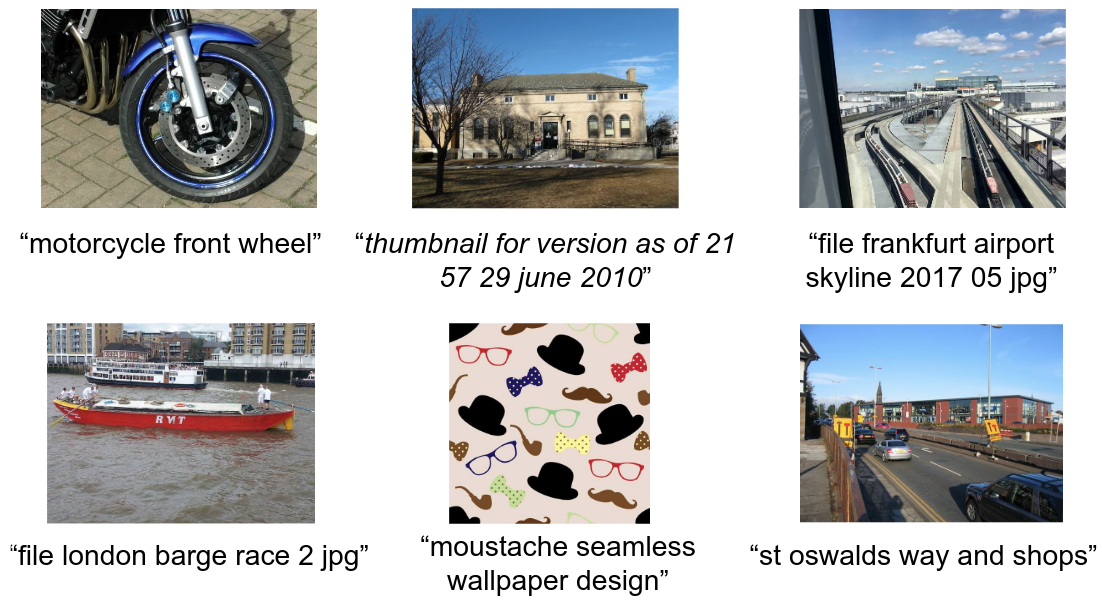
\includegraphics[width=\textwidth]{Images/crossmodalnetworks/examplepicsalign.png}
            \caption{Example of alt-text image pairs from the train dataset from \acrshort{align}}
            \label{fig:crossmodalnetworks:alignepairs}
        \end{figure}

        In a test for this paper, \acrshort{align} was much slower than CLIP to compute a zero-shoot evaluation on the CIFAR100\cite{cifar100} dataset.
        For 1 prediction, \acrshort{align} takes 70 times longer than \acrshort{clip} (see \cref{tab:clipaligntest}).
        Both networks are not fine-tuned. The highest predicted label is used. Due to the slow interference, ALIGN was stopped after processing 35\% of the dataset.

        \begin{table}
            \centering
            \begin{tabular}{lll}
                \hline
            \textbf{Measurment}&\textbf{ALIGN}&\textbf{CLIP}\\\hline
            Accuracy& 48.9\% & 61.7\%\\
            Speed(seconds per iterarion)&  2.16&  0.02\\ \hline
            \end{tabular}
            \caption{First test on CIFAR100.}
            \label{tab:clipaligntest}
        \end{table}

        \subsection{TinyCLIP
            \label{section:tinyclip}}
        \begin{figure}
            \centering
            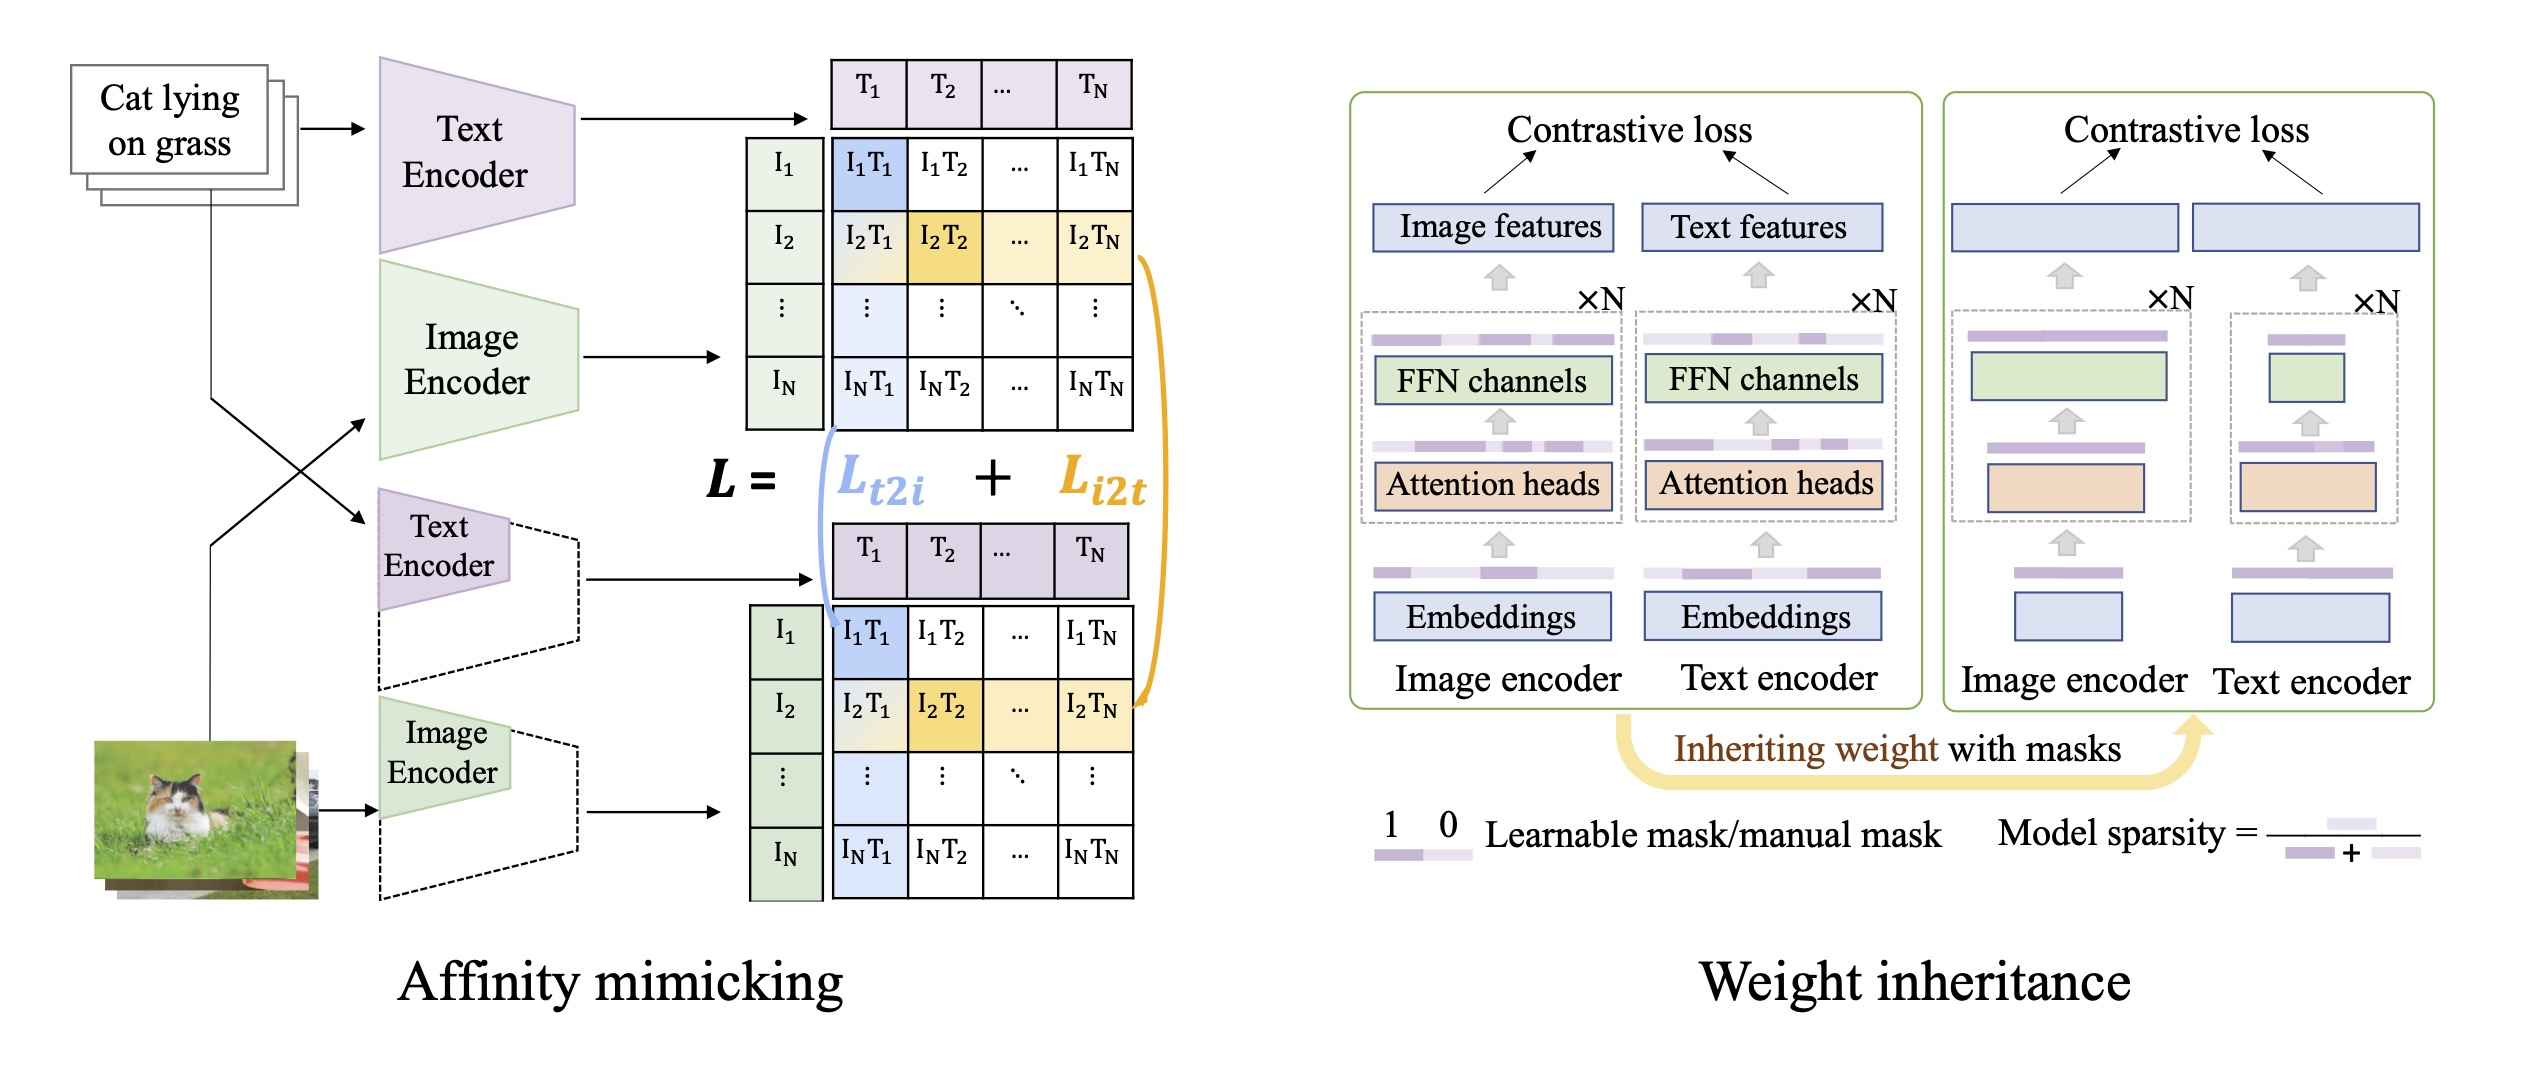
\includegraphics[width=\textwidth]{Images/crossmodalnetworks/TinyCLIP.jpg}
            \caption{Optimization which are used in TinyCLIP\cite{tinyclip}}
            \label{fig:crossmodalnetworks:tinyclip}
        \end{figure}

        TinyCLIP\cite{tinyclip} is a cross-modal distillation method for large-scale pre-trained speech-image models.
TinyClip can be used on limited systems due to its miniaturisation.
        It also speeds up training with minimal loss of model accuracy.
        It uses 3 concepts to reduce the size of the network.

        \subsubsection{Affinity mimicking}
        Affinity mimicking is a special form of knowledge distillation, also called model distillation.
        In knowledge distillation, a larger teacher network is trained first.
        After training the teacher network, a smaller student network is trained to predict the output of the teacher network.
        This works because the output of the teacher network has more information than the original label.
        Affinity Mimicking uses two new metrics in training: language-to-image loss and image-to-language loss (\(L_{t2i}\) and \(L_{i2t}\) in \cref{fig:crossmodalnetworks:tinyclip}).

        \subsubsection{Weight inhertiance}
        Weight inheritance is a technique that inherits important weights from well-trained teacher models to smaller student models.
        In the paper, the authors propose 2 methods:

        \subsubsection{Manual weight inhertiance}
        Based on the observations of the authors.
        Text encoders have most redundancy in depth (layer-wise), image encoders in width (channel-wise).
        They select \(k\) layers and channels of a branch, which will act as initialisation weights.
        To select the most important weights, some prior knowledge is required

        \subsubsection{Automatic weight inhertiance}
        The authors introduce a learnable mask to identify the importance of weight.

        \subsubsection{Multi-stage progressiv distillaiton}
        Pruning the model in several steps.
        For each stage, the authors use a modest degree of compression (e.g. 25\%). Each stage includes weight inheritance and affinity mimicking.

        % Due to the fact that TinyCLIP is already available and is much smaller in comparison to the origibal it will be further used in this work.

\section{Enhance the algorithm}

    To improve the accuracy of a pre-trained network, it can be fine-tuned to a specific task.
    Fine-tuning is a broad term.
    It ranges from the simple addition of a learnable linear layer at the end of the network to feature destillation.
    The concept of fine-tuning is derived from transfer learning\cite{transferlearning}.
    In transfer learning, the final layers of a neural network are removed and the network is retrained with new, independent layers.
    This saves time and resources.
    For example, with CLIP, a linear layer can be added to improve classification performance \cite{finetuneclip}.
    All of the fine-tuning approaches found use the output of the networks for further processing.
    Another way to increase the accuracy is to use better fitting text prompts.

    % \subsection{Probing}
    % % https://openaccess.thecvf.com/content/CVPR2024/papers/Huang_LP_A_Surprisingly_Strong_Linear_Probe_for_Few-Shot_CLIP_CVPR_2024_paper.pdf
    % \subsection{Feature destillation}
    % % https://arxiv.org/abs/2110.04544
    % \subsection{Prompt engeneering}

\section{Conclusion multi-modal networks}
    Based on the results of our own testing, ALIGN is not considered as a solution for this work.
    Instead, the focus of this work is on CLIP and TinyCLIP.
    These models can be fine-tuned to further improve their performance.
    In addition, the performance of the models can be improved by using better text prompts.